
% ===========================================================================
% Title:
% ---------------------------------------------------------------------------
% to create Type I fonts type "dvips -P cmz -t letter <filename>"
% ===========================================================================
\documentclass[11pt]{article}       %--- LATEX 2e base
\usepackage{amsmath,amsfonts,amssymb,amsthm,graphicx,graphics,epsf}
\setcounter{tocdepth}{3}
\usepackage{algorithmic}
\usepackage{algorithm}
\usepackage{hyperref,color}
\usepackage{comment}
\usepackage{url}
\usepackage{xspace}
\usepackage{booktabs}
\usepackage{latexsym}               %--- LATEX 2e base
%---------------- Wide format -----------------------------------------------
\textwidth=6in \textheight=9in \oddsidemargin=0.25in
\evensidemargin=0.25in \topmargin=-0.5in
%--------------- Def., Theorem, Proof, etc. ---------------------------------
\newtheorem{definition}{Definition}
\newtheorem{theorem}{Theorem}
\newtheorem{lemma}{Lemma}
\newtheorem{corollary}{Corollary}
\newtheorem{property}{Property}
\newtheorem{observation}{Observation}
\newtheorem{fact}{Fact}

\newcommand{\bit}{\text{bit}}
\newcommand{\depth}[1]{\ensuremath{d(#1)}}
\newcommand{\wlist}{ws-list\xspace}
\newcommand{\wlists}{ws-lists\xspace}

\newcommand{\halving}{Halving property\xspace}
\newcommand{\layer}{Layer property\xspace}

% ===========================================================================
\begin{document}
% ===========================================================================

% ############################################################################
% Title
% ############################################################################

\title{Working set dictionaries}


% ############################################################################
% Author(s) (no blank lines !)
\author{Luis Barba} % end-authors
% ############################################################################

\maketitle

\begin{abstract}
In this paper we develop a dictionary data structure, supporting insert and delete operations in $O(\log n)$ amortized time, while being able to search for an element $x$ in $O(\log w(x))$ amortized time. Here, $w(x)$ denotes the size of the working set of $x$, i.e., the number of elements that have been accessed in the structure since the last time $x$ was accessed. Moreover, the number of comparisons performed for this search is $(1+\delta)\log w(x) + O(1)$, where $\delta>0$ is an arbitrarily small constant. 
We present a lower bound in the comparison model showing that any comparison-based dictionary always contains an element $x$ such that at least $\log w(x) + \log\log w(x) - O(1)$ comparisons are required to search for $x$.
\end{abstract}

%%%%%%%%%%%%%%%%%%%%%%%%%%%%%%%%%%%%%%%%%%%%
\section{Introduction}
A dictionary is a data structure that stores a set of $n$ keys and supports insert, delete and search (access) operations.
There exist many structure for this purpose: AVL trees~\cite{adelsonvelskii1963algorithm}, Red-Black-trees~\cite{guibas1978dichromatic}, Splay-trees~\cite{sleator1985self}, among others. By using self-adjusting heuristics, Splay-trees provide a solution able to achieve $O(\log n)$ amortized time per operation, without storing any balance information at each node. Moreover, they are \emph{distribution-sensitive} dictionaries capable of performing better than $O(\log n)$ per operations by taking advantage of access patterns with certain distribution behaviors. 
This property presents itself in a variety of results regarding Splay-trees.

Let $X$ be a sequence of accesses to the $n$ elements stored in a dictionary.
Given a key $x$, let $f(x)$ be the frequency of accesses to $x$ in access sequence $X$. It was shown that, provided that the access distribution is known, it is possible to achieve a search time for element $x$ of $O(-\log f(x))$~\cite{hu1971optimal, knuth1971optimum} which matches the entropy bound~\cite{shannon1948mathematical}.
Trees achieving this bound are known as optimal search trees and have been improved to support insertion and deletion. However, they heavily rely on the knowledge of the access distribution beforehand. 
A seminal result of Sleator and Tarjan~\cite{sleator1985self} proves that Splay-trees share the same $O(-\log f(x))$ access time, only the bound is amortized, instead of worst-case. Surprisingly, they achieve this bound without prior knowledge of the acess distribution.
This property of Splay-trees was presented as the \emph{static optimality theorem}.

It was also shown that Splay-trees have the \emph{working set property}~\cite{sleator1985self}, which means that the time to search for an element is logarithmic in the number of distinct searches since this element was last accessed. 
Dictionaries with this property had been sought for by the research community~\cite{iacono2001alternatives, bose2008dynamic}, mainly 
because the working set property implies the static optimality theorem when sufficiently long sequences are considered~\cite{iacono2000improved}. 

The working set property is inspired in the following idea. If only a subset of $m$ elements is accessed, one would expect the time to search for an element to be $O(\log m)$, instead of $O(\log n)$. In fact, the working set property goes beyond this idea and states that searching for items that have been accessed recently should take less time. Formally, the \emph{working set} of $x$ is the set of distinct elements that have been accessed since the last time $x$ was search for, or since its insertion if it hasn't been searched for.
Let $w(x)$ be the number of elements in the working set of $x$. Any dictionary with the \emph{working set property} should be able to search for $x$ in time $O(1 + \log w(x))$. 


While Splay-trees have the working set property, an access for $x$ takes $O(1+\log w(x))$ amortized time, rather than worst-case. A dictionary achieving a worst-case performance while retaining the working-set property was presented by Iacono in~\cite{iacono2001alternatives} and is revisited in this paper. 
Inspired in this structure, Bose, Howat and Morin presented a binary search tree with the working set property~\cite{bose2010layered}.

Trying to obtain low space overhead data structures, Bose \emph{et. al}~\cite{bose2012distribution} showed how to construct a dictionary, with the working set property, such that the space overhead of this structure is $O(\log \log n)$, i.e., only $O(\log\log n)$ additional variables (each of size $O(\log n)$ bits) are stored aside from the data itself.


In this paper we measure the efficiency of a dictionary in a different way. The \emph{cost} of an access in a comparison-based data structure is the number of comparisons made by any search algorithm in this structure.
Both Splay-trees and Iacono's working set data structure are comparison-based structures, i.e., their search algorithms can be encoded as a decision tree where each node represents a comparison and its children the possible outputs of that comparison. 
Moreover, each leaf represents a different output for the search query. 
In Section~\ref{section:Comparing searching costs}, we compare the cost of an access in Splay-trees and in Iacono's working set structure. In Section~\ref{section:New structure}, we present a new data structure, based on skip-lists, where the cost of searching for an element $x$ is $(1+\delta) \log w(x) + O(1)$, for any constant $\delta>0$. Finally, in Section~\ref{section:Lower Bounds} we present a lower bound on the cost of an access on any comparison-based dictionary that has the working-set property. In other words, we prove that in any such structure, there is always an element $x$ where the cost to search for $x$ is at least $\log w(x) + \log\log w(x) - O(1)$. 


%Queueish set properties

%%%%%%%%%%%%%%%%%%%%%%%%%%%%%%%%%%%%%%%%%%%%
\section{Searching costs}\label{section:Comparing searching costs}
In this section, we analyze the cost of a search in Splay-trees and in Iacono's working set data structure, i.e., we count the number of comparisons required to find an element in these structures. 
For the moment, we assume 3-way comparisons that determine, in one atomic operation, if the first of the compared items is either smaller, equal or larger than the second one. Later in Section~\ref{section:2-way comparisons}, we explore the cost of searching using 2-way comparisons, i.e., to test for equality two comparisons are needed.

Given a set $S= \{x_1, \ldots, x_n\}$ stored in a dictionary, we can assume that the working set sizes of the elements in $S$ define a permutation of $n$. That is, no two elements have the same working set and for every $1\leq i\leq n$, there is an element $x$ of $S$ such that $w(x) = i$.

\subsection{Cost of searching in Splay-trees}

In a Splay-tree, every node is arbitrarily assigned a positive weight.
The size of a node $x$ in the Splay-tree, denoted by $s(x)$, is the sum of all individual weights of the nodes in the sub-tree rooted at $x$. Let $r(x) = \log s(x)$ denote the \emph{rank}  of $x$ in the tree and define the potential of a Splay-tree as the sum of the ranks of all its nodes.

\begin{lemma}\label{lemma:Access lemma}(\textsc{Access Lemma}~\cite{sleator1985self})
The amortized time to splay a tree with root $t$ at a node $x$ is at most $3(r(t) - r(x)) + 1$.
\end{lemma}

To prove the working set property for Splay-trees, we fix the weight of any item $x$ to be $1/w(x)^{1+\varepsilon}$, for an arbitrarily small constant $\varepsilon > 0$.
Therefore, if $t$ denotes the root of a Splay tree $T$, $r(t) = \log (\sum_{x\in T} 1/w(x)^{1+\varepsilon}) = \sum_{i=1}^n  1/i^{1+\varepsilon}$ as the working sets sizes define a permutation of $n$. Thus, $r(t) = c_\varepsilon$ is a constant depending only on $\varepsilon$.
By Lemma~\ref{lemma:Access lemma}, the amortized cost of splaying after searching for $x$ is $3(r(t) - r(x)) = 3(c_\varepsilon - r(x)) = 3c_\varepsilon - 3\log s(x)$. Since $s(x) \geq \frac{1}{w(x)^{1+\varepsilon}}$, we get that $r(t) \leq  3c_\varepsilon - 3\log \frac{1}{w(x)^{1+\varepsilon}}  = O(1)_\varepsilon + 3\cdot (1+\varepsilon)\log w(x)$, where the constant hidden by the big $O$ notation depends on $\varepsilon$. 
After accessing an element, we need also to account for the change in potential as weights are readjusted. 
Since $w(x)$ becomes 1 after accessing $x$, the weight of $x$ increases to 1. Furthermore, the weight of every node $y$ decreases to $1/(w(y) +1)^{1+\varepsilon}$ if $y$ was in the working set of $x$ prior to the access.
As the size of the root is unchanged, the weight reassignment changes the potential in at most $\log (1)- \log s(x) = - \log \frac{1}{w(x)^{1+\varepsilon}} = (1+\varepsilon)\log w(x)$. 
We obtain the following.

\begin{lemma}\label{lemma:Splay-trees cost}
The total cost of searching for an element $x$ in a Splay-tree is at most \linebreak $O(1)_\varepsilon + 4\cdot (1+\varepsilon)\log w(x)$ for any constant $\varepsilon > 0$.
\end{lemma}





%%%%%%%%%%%%%%%%%%%%%%%%%%%%%%%%%%%%%%%%%%%%
\subsection{Cost of searching in Iacono's working set structure}

To store a dynamic set $S$ of $n$ elements, Iacono's working set structure~\cite{iacono2001alternatives} consists of a series of Red-black trees~\cite{guibas1978dichromatic}, or other Self-balancing binary search trees $T_1, T_2, \ldots, T_k$, and a series of deques (Double-ended queues) $Q_1, Q_2, \ldots Q_k$, where $k = \lceil \log \log n\rceil$. 
For every $1\leq i\leq k$, tree $T_i$ and deque $Q_i$ share the same contents and pointers are maintained between their corresponding elements. For every $ i < k $, the size of $T_i$ and $Q_i$ is $2^{2^i}$. Tree $T_k$ and deque $Q_k$ consist of the remaining elements, i.e.,  their size is $n - \sum_{i=1}^{k-1} 2^{2^i}$. Therefore, the number of items in all trees and the number of elements in all deques both add up to $n$.
Every element that has been inserted in the data structure is stored in exactly one of the trees and its corresponding deque. 

\textbf{Working set Invariant.}
In the deques of this structure, elements are kept in sorted order according to their working set size.
Formally, element $x$ lies after $y$ in deque $Q_i$ if and only if $w(x)< w(y)$. Moreover, for every $1\leq i < k$, the elements in deque $Q_i$ have smaller working sets than the elements in deque $Q_{i+1}$. This property is referred to as the Working set invariant. Every operation in the data structure maintains the Working set invariant.

\subsubsection*{Operations}
The basic operation in this structure is called shift from $h$ to $j$, where $h$ and $j$ are indices of some trees in the structure. 
Two cases are considered in a shift from $h$ to $j$: If $h< j$, then for every $h\leq i < j$, taken in increasing order, an item is dequeued from $Q_i$ and enqueued into $Q_{i+1}$. The corresponding item is deleted from $T_i$ and inserted into $T_{i+1}$. The running time of this operation is $O(\sum_{i=h}^{j} \log_2 |T_i|) = O(\sum_{i=h}^{j} \log_2 2^{2^i}) = O(2^j)$. 
Analogously, if $ j< h$, then for every $j < i \leq h$, taken in decreasing order, an item is dequeued from $Q_i$ and enqueued into $Q_{i-1}$. The corresponding item is deleted from $T_i$ and inserted into $T_{i-1}$. The running time of this operation is $O(\sum_{i=j}^{h} \log_2 |T_i|) = O(\sum_{i=j}^{h} \log_2 2^{2^i}) = O(2^ h)$. 
Regardless of the case, after a shift operation, the size of $T_h$ decreases by one whereas the size of $T_j$ increases by one.
Since elements in the deques are sorted with respect to their working sets sizes, a shift operation maintains the Working set invariant. We proceed to analyze a search operation.


\subsubsection*{Search} 
To search for an element $x$, search for $x$ in $T_1, T_2, \ldots T_k$, in increasing order, until finding a tree $T_j$ containing $x$. If no tree is found, the search is unsuccessful. If $x$ is found, it is deleted from $T_j$ and then inserted into $T_1$, i.e., it is moved to the front of the structure. The search finishes by performing a shift from $1$ to $j$ which restores the size of every tree and every deque to their size prior to the search operation.

Assume that $x$ lies at depth $\log_2 |T_j|$ in $T_j$ since we want to find a lower bound on the maximum cost of a search.
Thus, the cost of a successful search for $x$ is $\sum_{i=1}^j 2^i = \frac{2(2^j -1)}{2-1} = 4(2^{j-1} - 1/2)$ as one comparison is made at each visited node in every $T_i$.
By the Working set property, every element in the working set of $x$ lies in trees $T_1, \ldots, T_{j-1}$. 
In the worst case, $x$ could be the element in $T_j$ with the smallest working set and hence, $w(x) = 2^{2^{j-1}}+1$, implying that $\log w(x) = 2^{j-1}$.
Consequently, in the worst case, the cost of a search for $x$ is at least $4(2^{j-1} - 1/2) = 4 (\log w(x) - 1/2)$. 

\begin{lemma}\label{lemma:Iacono's structure cost}
In the worst case, the total cost of searching for an element $x$ in Iacono's working set structure is at least $4 \log w(x) - O(1)$.
\end{lemma}


%%%%%%%%%%%%%%%%%%%%%%%%%%%%%%%%%%%%%%%%%%%%
\section{Working set skip lists}\label{section:New structure}
In this section, we present  a \wlist which is a comparison-based dictionary with the working set property. 
We prove that for any constant $\delta>0$, the cost of searching for an element $x$ in a \wlist is at most $(1+\delta)\log w(x) + O(1)$. Therefore, achieving a leading constant on the main term arbitrarily close to one, as opposed to Splay-trees and the working set structure which require $4\log w(x)$.

Let $S$ be a set of $n$ numbers.
For any fixed constant $0 < \varepsilon < 1/2$, let $a = 2-\varepsilon$ and let $k = \lceil \frac{\log n}{\log a}\rceil$. 
A \emph{\wlist} is based on the same paradigm as skip-lists~\cite{pugh1990skip} and consists of $k+1$ levels.
 
Each node $v$ in a \wlist has a pointer $v.key$ to an element of $S$ called the \emph{key} of $v$. 
Given a node $v$ in a list, if $v.key$ points to element $x$ of $S$, we say that $x$ is \emph{represented} in this list by $v$.
For each $0\leq i\leq k$, level $i$ stores a sorted list $L_i$ of nodes.
Thus, the set of nodes in $L_i$ maps to a subset of $S$.
In addition, we store a global list $W$ with a node for each element of $S$.
We enumerate some properties that \wlist will have. 
\begin{itemize}
\item List $W$ is a sorted list of nodes with respect to the working set size of their keys.
\item Every element $x$ of $S$ has a pointer to the node in $W$ that represents it.
\item List $L_i$ is a sorted list of nodes with respect to their keys.
\item If an element $x$ of $S$ is represented in $L_i$, then it is also represented in $L_{i+1}$. 
\item Every element of $S$ is represented in $L_k$. 
\item No element of $S$ is represented twice in the same level. 
\end{itemize}

\pagebreak
Additionally, two main properties are maintained on every level $i$ of a \wlist.
\begin{itemize}
\item \textbf{\halving.} For any two consecutive nodes in list $L_i$, at least one of them has its key represented in list $L_{i-1}$.
\item\textbf{\layer.} Every element of $S$ with working set smaller than $a^i$ is represented in list $L_i$.
\end{itemize}


Given a node $v$ in a list, we use $v.next$ to represent its successor in this list.
Since level $k$ defines the largest list $L_k$ having a node for every element in $S$, we can construct it in $O(n\log n)$ time after sorting the elements of $S$ by key. 
In the same way, list $W$ can be constructed after sorting the elements of $S$ by the size of their working set. 
Double-linked pointers are maintained between the elements of $S$ and the nodes in $W$ that represent them.
In addition, a node $w$ in $W$ has an extra pointer $w.aux$ that will be updated in every construction step.

The rest of the levels are constructed using procedure \textsc{LevelConstruction} which accepts a sorted list $L_{i+1}$ as input, where $i < k$. 
Procedure \textsc{LevelConstruction} constructs a new lists $L_{i}$  from $L_{i+1}$ and $W$.
The idea is to choose one out of every two nodes of list $L_{i+1}$ and ``copy'' them to list $L_i$.
In addition, $L_i$ will also contain a node for each element of $S$ that has working set size at most $a^i$.

A  \emph{copy} of a node, is a new node that uses the same key.
Nodes at level $i$ of the \wlist will keep a $down$ pointer to the element in $i+1$ that shares a key with this node.
We proceed to describe the construction procedure.

\subsubsection*{LevelConstruction}
Traverse list $L_{i+1}$ in order by following $next$ pointers. For each vertex $v$ visited, let $w$ be the node in $W$ that represents $v$'s key.
Update the auxiliary pointer at $w$ by letting $w.aux$ point to $v$. 
Thus, $|L_{i+1}|$ nodes of $W$ were updated. 
Moreover, if we assume that $L_{i+1}$ has the \layer, then every node in $W$ whose key has working set size smaller than $a^{i+1}$ was updated.

Traverse $W$ in order, starting with the node whose key has the smallest working set and stopping when reaching the $\lfloor a^i\rfloor$-th node. 
Since every visited node $w$ of $W$ was updated in the previous step, we can follow its $aux$ pointer and \emph{mark} node $w.aux$ in $L_{i+1}$. 

To construct $L_i$, start with an empty list. Then, traverse $L_{i+1}$ in order and keep track of the rank of the visited nodes in $L_{i+1}$.
When traversing a node $v$, if either $v$ has odd rank or was marked in the previous step, then create a copy $u$ of $v$.
Let $u.down$ point to $v$ and append $u$ at the end of $L_i$. 
Since nodes are inserted in $L_i$ as they are traversed in $L_{i+1}$, nodes in $L_i$ appear in the same order as they appear in $L_{i+1}$.\\

\begin{figure}[tb]
\centering
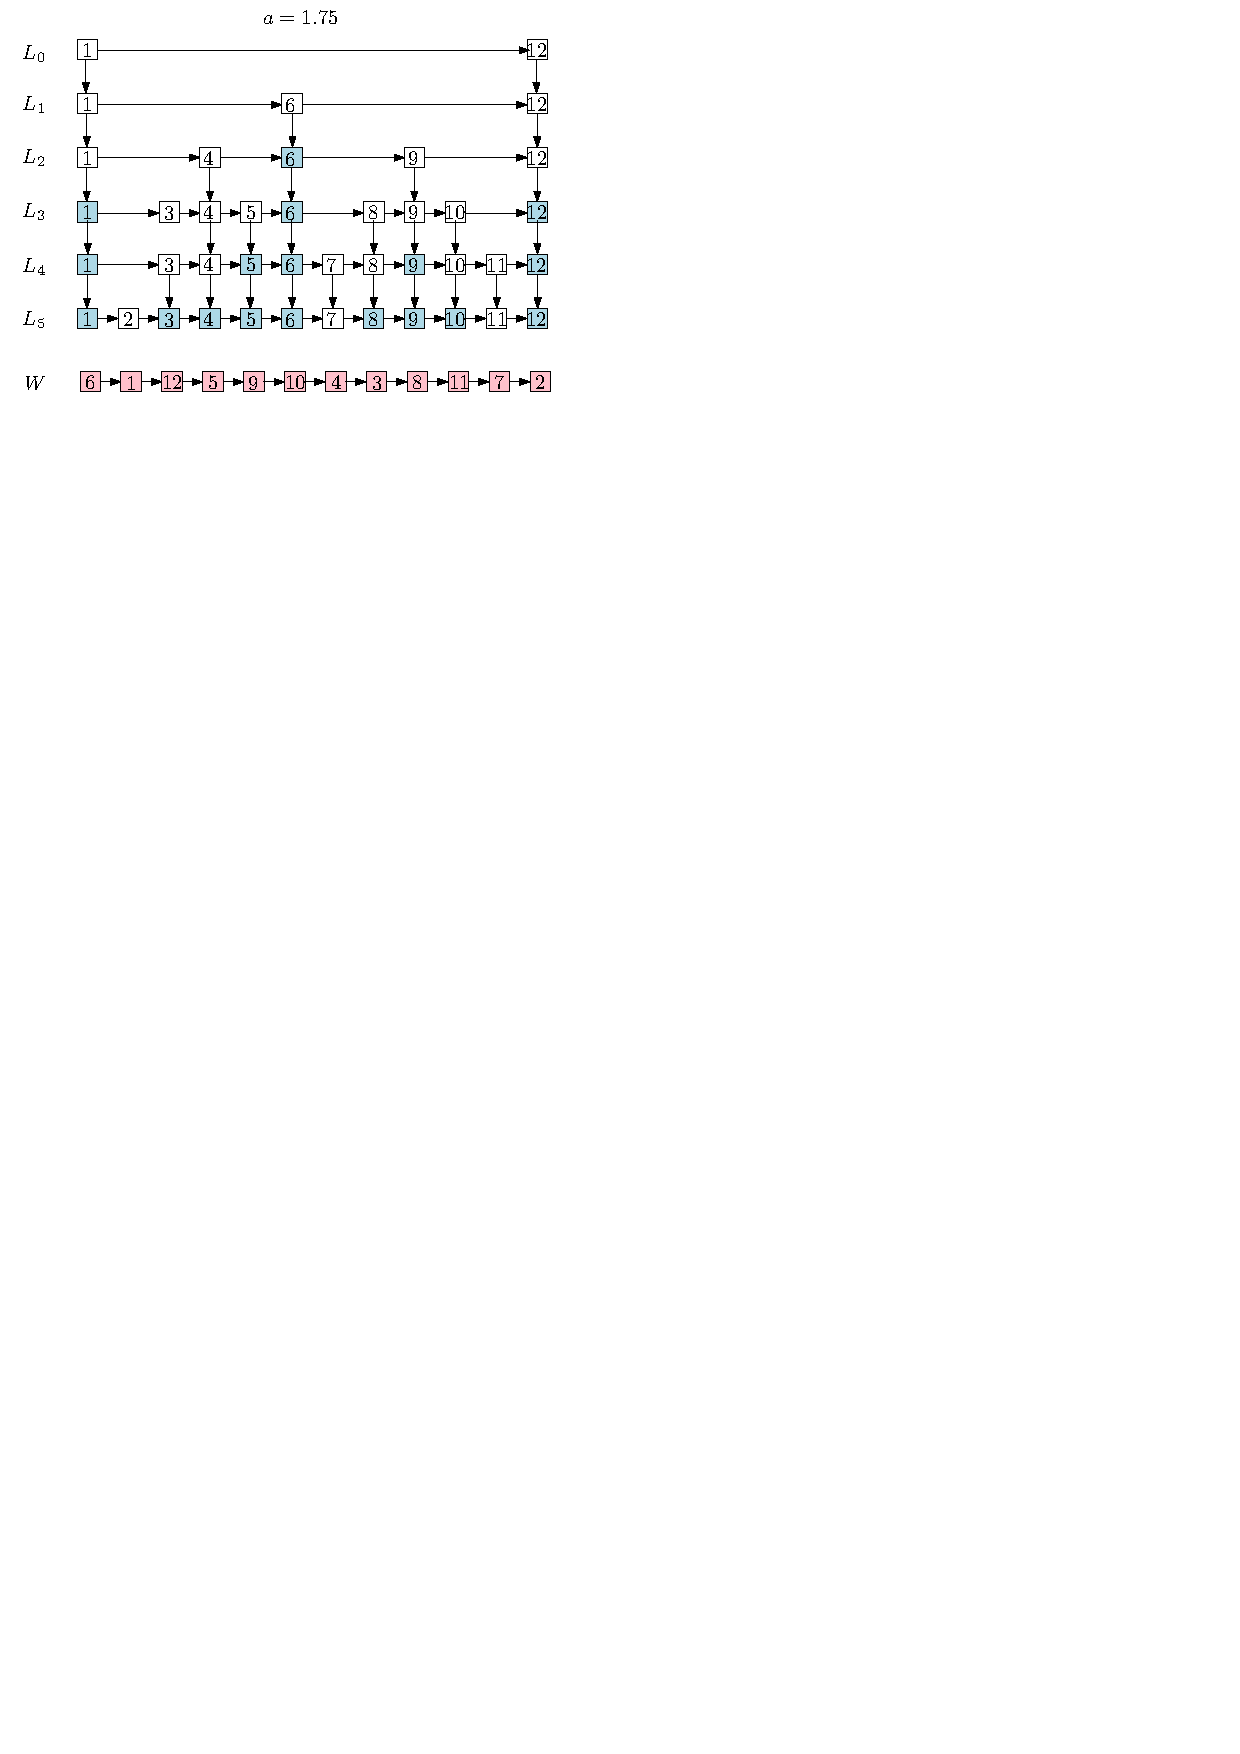
\includegraphics{img/wlist.pdf}
%[width=1\textwidth]
\caption{\small A \wlist with 12 elements constructed by picking $a = 1.75$, i.e., $\varepsilon = 1/4$. List $W$ keeps nodes sorted by the working set size of their keys. Nodes in each $L_i$ are sorted by their key. List $L_i$ consists of every element in $L_{i+1}$ with odd rank plus all nodes representing elements whose working set size is smaller than $a^i$. Elements in blue in list $L_{i+1}$ have working set size smaller than $a^i$ and need to be copied into $L_i$.}
\label{fig:Wlist}
\end{figure}

Given a list $L_t$, we perform a \emph{rebuild at level $t$} by discarding all levels smaller than $t$ (if any). 
Then, we build levels $t-1, t-2, \ldots, 1$ using recursive calls to \textsc{LevelConstruction}. 
Formally, for every $0\leq i< t$, list $L_i$ is defined as the output of procedure \textsc{LevelConstruction} with input $L_{i+1}$.

To construct a \wlist, invoke a rebuild at level $k$ after creating lists $L_k$ and $W_k$ in $O(n\log n)$ time; see Fig.~\ref{fig:Wlist} for an illustration.

\pagebreak
\begin{lemma}\label{lemma:Properties of Level rebuild}
Given a list $L_t$ in a \wlist where the \layer and the \halving hold, a rebuild at level $t$ constructs new lists $L_0, \ldots, L_{t-1}$ in $O(|L_t|)$ time, using no comparisons. Moreover, $\sum_{i=1}^{t-1} |L_i| = O(|L_t|)$ and for every $1\leq j < t$ it holds that:
\begin{itemize}
\item The size of list $L_j$ is at most $\left\lceil\frac{|L_{j+1}|}{2}\right \rceil + a^j$.
\item Nodes in list $L_j$ are sorted by their keys.
\item Both the \halving and the \layer hold at level $j$.
\end{itemize}
\end{lemma}
\begin{proof}
The construction invokes procedure \textsc{LevelConstruction} recursively, starting with input $L_t$. 
It produce a sequence of lists $L_0, \ldots, L_{t-1}$ where each $L_j$ is constructed from $L_{j+1}$ using \textsc{LevelConstruction}. 
Consider two consecutive nodes $v_i$ and $v_{i+1}$ in list $L_{j+1}$. 
One of them will have an odd rank in list $L_{j+1}$ and hence, it will be copied and its key will be represented in list $L_j$. 
Thus, the \halving holds.

When constructing $L_j$, the first $a^{j}$ nodes in $W$ helped mark their corresponding nodes in $L_{j+1}$ which were then copied into $L_j$. 
Thus, each element with working set smaller than $a^j$ is represented in $L_j$, provided that every element with working set smaller than $a^{j+1}$ is represented in $L_{j+1}$. Therefore, the \layer holds on every level.
Nodes in $L_j$  are copied in order with respect to their key, provided that the nodes in $L_{j+1}$ are sorted by their key. 

To construct list $L_j$, we traversed list $L_{j+1}$ twice as well as the first $a^j$ nodes of list $W$. 
Since nodes are always added to $L_j$ at the end of the list, we can construct $L_j$ in $O(|L_{j+1}| + a^j) = O(|L_{j+1}|)$ time.
Therefore, the total time required to construct lists $L_0, \ldots, L_{t-1}$ is $O(\sum_{j=0}^{t-1} |L_{j+1}|)$.
Because half of the nodes in $L_{j+1}$ are copied to list $L_j$, and at most $a^j$ additional nodes are also copied, we know that $|L_j| \leq \lceil |L_{j+1}|/2\rceil + a^j$
Therefore, one can prove inductively that $O(\sum_{j=0}^{t-1} |L_{j+1}|) \leq O(|L_t| + 2\sum_{j=0}^{t-1} a^j)$.
Notice that $\sum_{j=0}^{t-1} a^j = O(a^t)$. Moreover, $|L_t| > a^t$ as the \layer holds at level $t$.
Consequently, the total running time of a rebuild at level $t$ is $O(|L_t| + 2\sum_{j=0}^{t-1} a^j) = O(|L_t| + a^t) = O(|L_t|)$.
Furthermore, the same argument can be used to prove that, after a rebuild at level $t$ is performed, the size of the first $t-1$ levels adds up tho $O(|L_t|)$.
Since no data comparison is done by procedure \textsc{LevelConstruction}, our result follows.
\end{proof}

%By Lemma~\ref{lemma:Properties of Level rebuild}, we know that we can construct a \wlist  by invoking a rebuild at level $k$ after constructing lists $L_k$ and $W_k$ in $O(n\log n)$ time; see Fig.~\ref{fig:Wlist} for an illustration.
%Moreover, the size of the structure is $O(|L_k|) = O(n)$.

Recall that $a = 2-\varepsilon$ for some fixed constant $0<\varepsilon < 1/2$. The next result guarantees that the size of list $L_0$ is ``small'' after a rebuild.

\begin{lemma}\label{lemma:Size at level zero}
If $|L_t| < 2^t$ for some level $0< t\leq k$, then after a rebuild at level $t$ the size of $L_0$ is at most $c_a = 1 +\frac{1}{1-2^{\log (a/2)}}= O(1)$.
\end{lemma}
\begin{proof}
After the level rebuild, $|L_i| \leq \lceil |L_{i+1}|/2 \rceil + a^i$ for every $0\leq i< t$. Therefore, the size of $L_0$ can be expanded as follows.
$$|L_0| \leq \frac{|L_t|}{2^t} + \sum_{i=0}^{t-1} \frac{a^i}{2^i}\leq \frac{2^t}{2^t} + \sum_{i=0}^{t-1} \frac{a^i}{2^i}.$$
Note that $\frac{a^i}{2^i} = 2^{i \log (a/2) }$. Because $\log a <1$, we get that $\log a -1 = \log (a/2) < 0$ and hence, $2^{\log (a/2)} <1$. By the properties of the geometric series, we get that
$$|L_0| \leq 1 + \sum_{i=0}^{t-1} 2^{i \log (a /2)} = 1 + \sum_{i=0}^{t-1} (2^{\log (a/2)})^i < 1 +\frac{1}{1-2^{\log (a/2)}} = c_a.$$
\end{proof}


\subsection{Searching in \wlists}

Since every element that is represented in $L_i$ is also represented in $L_{i+1}$, every node $v$ of $L_i$ holds pointers $v.next$ to a node in $L_i$ and $v.down$ to the node in $L_{i+1}$ that shares its key with $v$.

To search for element $x$ in a \wlist, let $i = 0$ and define your starting node as the the first node of $L_0$.
Walk list $L_i$ from the starting node, by following $next$ pointers, until finding a node $v$ such that $x$ is larger or equal than $v.key$ but smaller than the key of $v.next$. If $v.key$ is equal to $x$ finish and report the element where $v.key$ points to.
Otherwise, jump to the next level by following pointer $v.down$ and restart the search starting from $v.down$ in list $L_{i+1}$.
If we reach the last node of list $L_k$, report that $x$ does not belong to the \wlist.

In this algorithm, a (3-way) comparison is made to decide which pointer to follow on each step of the algorithm.
Therefore, the cost of a search is equal to the number of pointer jumps performed. The set of nodes visited during  a search is called a \emph{search path}; see Fig.~\ref{fig:Promotion} for an illustration of a search path.

For ease of description, we say that a node $u$ is \emph{smaller} than node $v$ (denoted by $u<v$) if $u.key < v.key$. Similarly, we say that $u$ is smaller than some number $y$ if $u.key < y$.
The \emph{depth} of an element $x$ of $S$ in a \wlist is the smallest index $i$ such that $x$ is represented in list $L_i$.
We obtain the following result.


\begin{lemma}\label{lemma:Visited Nodes}
If a \wlist has the \halving, then at most $|L_0| + 2(t-1)$ nodes are visited in a successful search, where $t$ is the depth of the searched element.
\end{lemma}
\begin{proof}
In the worst-case, the algorithm may scan the whole list $L_0$ before following a $down$ pointer. Therefore, in the worst-case $|L_0|$ nodes will be visited before leaving level 0.

Assume that at least three nodes are visited at some level $i>0$ when searching for an element $x$. 
Therefore, there exists a node $v$ in list $L_i$, such that $v<v.next < v.next.next < x$ and $v$ was reached by a $down$ pointer from some node $u$ in $L_{i-1}$. 

Since we followed the $down$ pointer from $u$, we know that $x$ is smaller than $u.next$. 
However, $x$ is larger than $v.next$ and $v.next.next$. Notice that if there was a node $w$ in $L_{i-1}$ such that $w.down$ points to $v.next$, then $w$ needs to lie after $u.next$ or before $u$ in $L_{i-1}$. 
Because $w.key = v.next.key$, we know that $w$ is smaller than $u.next$ and larger than $u$. A contradiction since nodes in $L_{i-1}$ are sorted according to their key. The same happens if there was a node in $L_{i-1}$ pointing down to $v.next.next$. 
Therefore, no node in $L_{i-1}$ has a $down$ pointer to $v.next$ nor to $v.next.next$. This violates the \halving since the keys of $v.next$ and $v.next.next$ are not represented in $L_{i-1}$. 
We conclude that, if the \halving holds and $t$ is the depth of $x$ in the \wlist, then at most two nodes are visited on each level $1\leq i\leq t$ before finding $x$.
\end{proof}

By Lemma~\ref{lemma:Visited Nodes}, we can implement search on a \wlist in a succinct way using at most one comparison on each list above $L_0$.
Pseudo code for this algorithm can be found in Algorithm~\ref{alg:Working set skip list Search}.

\begin{corollary}\label{corollary:SearchCost}
If a \wlist has the \halving, then the cost to search for an element is at most $|L_0| + t$, where $t$ is the depth of the searched element.
\end{corollary}

\begin{algorithm}
  \begin{algorithmic}[1]
    \STATE Let $v\gets$ smallest element in $L_0$.
    \WHILE{$v.next.key < x$}
    	\STATE $v\gets v.next$.
    \ENDWHILE 
    \STATE Let $v\gets v.down$.
    \WHILE{$v$ is not the last element in $L_k$}
	\IF{$v.next.key = x$}\label{step:equality}
		\STATE Report $v.next.key$ and finish.
	\ELSIF{$v.next.key > x$}
		\STATE $v\gets v.down$.
	\ELSIF{$v.next.key  < x$}
		\STATE $v\gets v.next.down$.
	\ENDIF
    \ENDWHILE
    \STATE Finish and report an unsuccessful search.
  \end{algorithmic}
\caption{Given an element $x$ of $S$, algorithm to search for $x$ in a \wlist with the \halving.}
\label{alg:Working set skip list Search}
\end{algorithm}

\begin{figure}[tb]
\centering
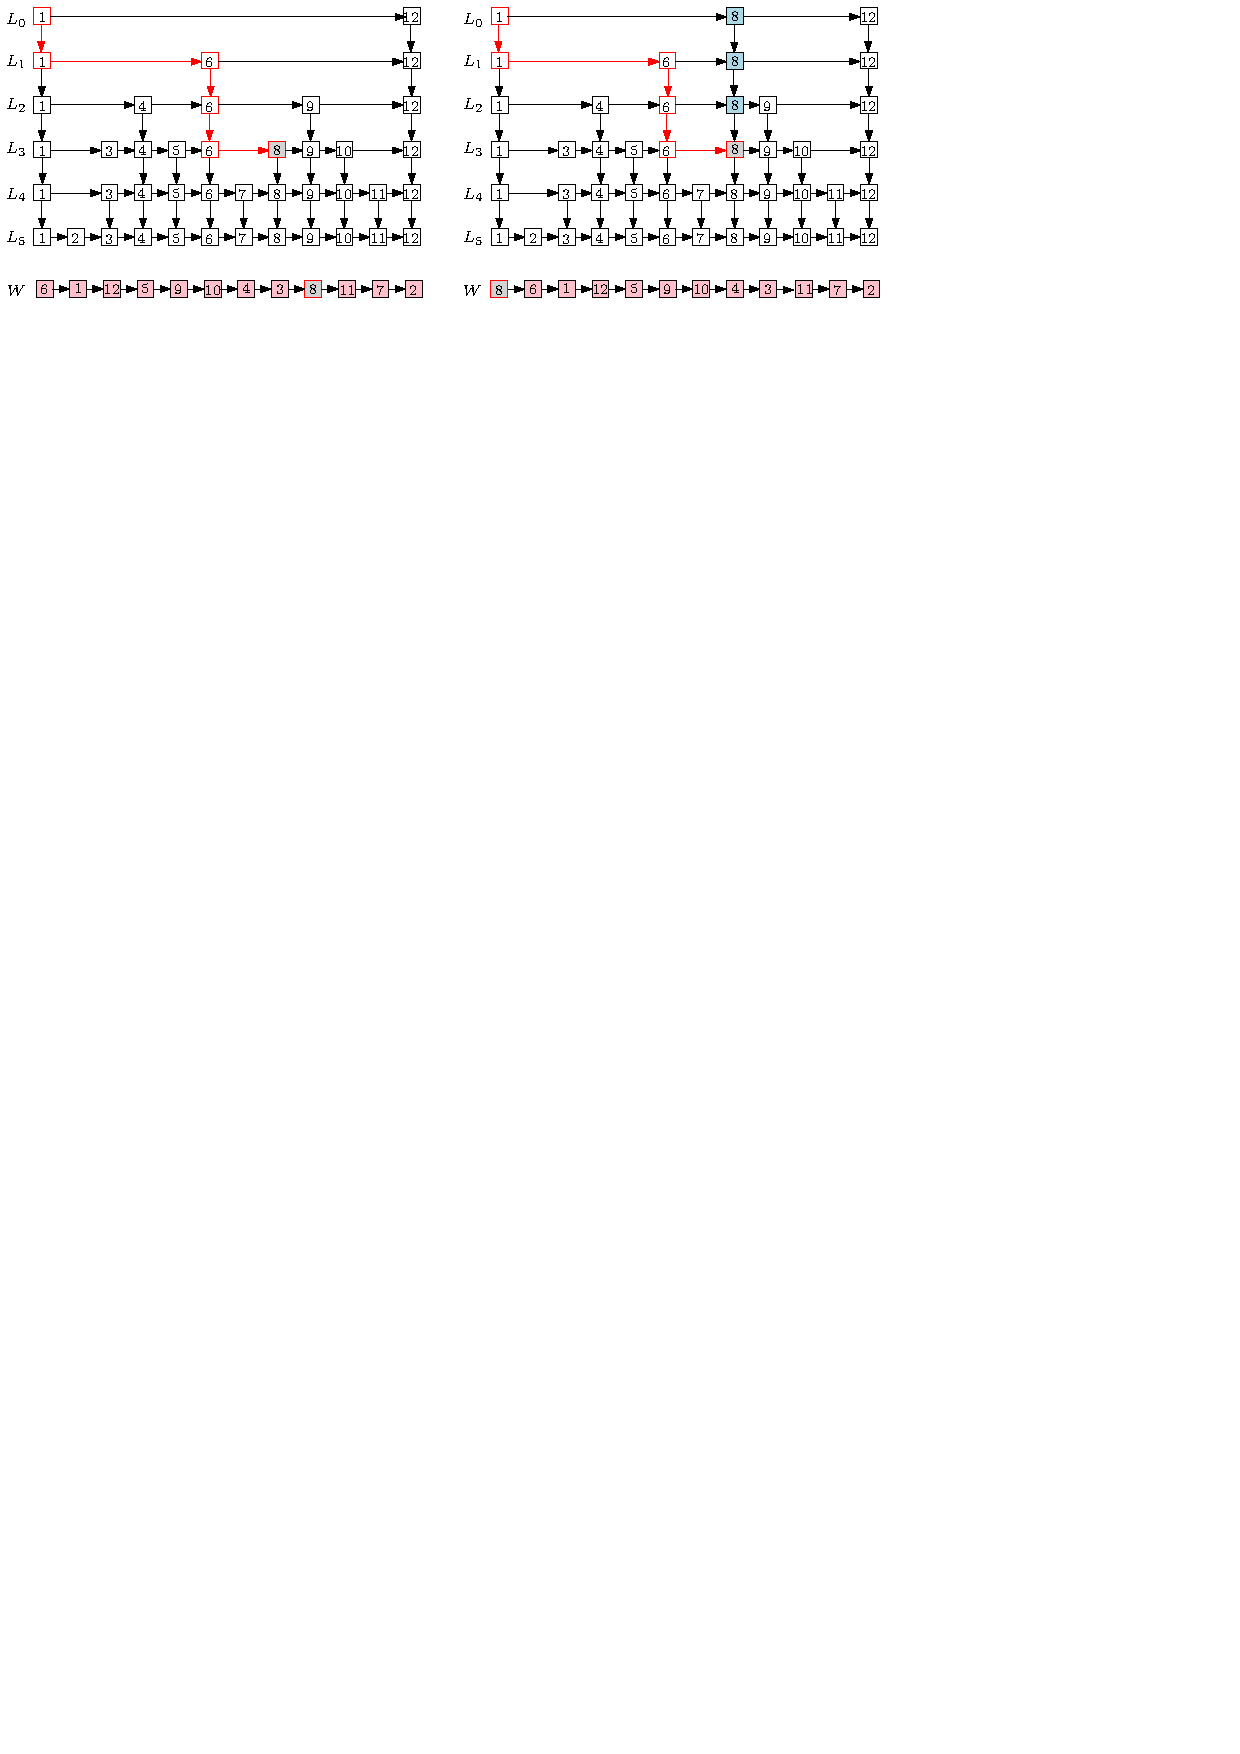
\includegraphics[width=1\textwidth]{img/Promotion.pdf}
\caption{\small A search for element $8$ in a \wlist. To the left, the search path is depicted in red and the first node found that represents $8$ is shown in gray. To the right, the promotion of $8$ to the top by creating three nodes shown in blue. Each of these nodes is spliced,  on each level, to the right of the level-maximum elements in this search path. The node representing $8$ in $W$ is pushed to the beginning of list.}
\label{fig:Promotion}
\end{figure}

\subsection{Working set property}

By Corollary~\ref{corollary:SearchCost}, we know that if the \halving is maintained, then the cost to search for an element is at most its depth plus the size of $L_0$. Consequently, to have the working set property, we want recently accessed elements to be represented in the lower levels of the \wlist, while elements last accessed long time ago appear in higher levels. 
To prove the working set property, we rely on the \layer.

\begin{lemma}\label{lemma:Layer property}
If a \wlist has the \layer, then the depth of element $x\in S$ in the \wlist is at most $\frac{\log w(x)}{\log a} + 1$.
\end{lemma}
\begin{proof}
Given an element $x$ of $S$, let $i$ be the smallest index such that $L_{i}$ contains element $x$. Because $x$ is not in $L_{i-1}$, by the \layer we know that $w(x) > a^{i-1}$. Therefore, $\log w(x) > (i-1)\log a$ which implies that $i <\frac{\log w(x)}{\log a} + 1$.
\end{proof}

By Corollary~\ref{corollary:SearchCost} and Lemma~\ref{lemma:Layer property}, we obtain the following result.

\begin{corollary}\label{corollary:Cost of search}
If the \halving and the \layer are maintained, then the cost to search for element $x$ is at most $|L_0| + \frac{\log w(x)}{\log a} + 1$.
\end{corollary}

\subsection{Maintaining invariants in a \wlist}
By Corollary~\ref{corollary:Cost of search} if a \wlist has the \halving, the \layer and keeps the size of $L_0$ ``small'', then it has the working set property. 

Assume that we are given a \wlist where $|L_0| = O(1)$, and both the \layer and the \halving hold. We want to maintain these properties after a successful search for an element $x$ in this \wlist. Notice that the working set size of $x$ becomes one after accessing this element. 
To fix the order in $W$, consider the node representing $x$ in this list. Remove this node from its location and then insert it at the beginning of $W$.
Besides fixing $W$, if $x$ was found at level $t>0$ in the \wlist, we still have a violation of the \layer.
Let $u_t$ be the node in list $L_t$ where $x$ was found.
Let $\{v_0, v_1, \ldots, v_{t-1}\}$ be a subset of the search path of $x$ such that, for $0\leq i<t$, $v_i$ is the largest node visited in list $L_i$ that is smaller than $x$. 
We can store this set as we traverse the \wlist during a search for $x$.

To reestablish the \layer, we \emph{promote} $x$ to the top of the \wlist as follows. For every $0\leq i < t$, splice a new node $u_i$ with key $x$ between $v_i$ and $v_i.next$. Moreover, add pointers between newly created nodes if they lies in consecutive layers, i.e., let $u_i.down$ point to $u_{i+1}$; see Fig.~\ref{fig:Promotion} for an illustration. 
Intuitively, we make sure that recently accessed elements are represented in the top levels of the structure.

After promoting $x$, it is represented on every level of the structure, in particular at level $L_0$. 
Therefore, the size of $L_0$ increases by one. 
By Corollary~\ref{corollary:SearchCost}, we need for $L_0$ to have constant size to keep the cost of a search in the desired range.
In particular, we want the size of $L_0$ to be at most $c_a = 1+\frac{1}{1-2^{\log (a/2)}}$ where $a = 2-\varepsilon$. 
If at any point $|L_0| > c_a$, we rebuild the ``top'' part of the structure to bring the size of $L_0$ down. 
To do that, let $b= 2-\varepsilon/2$ be a constant greater than $a$ but smaller than 2.
If $|L_0| > c_a$, we find the first index $t$ such that $|L_t| < b^t$. 
Such an index always exists because $|L_0| > b^0$ and $|L_k| = n = a^k < b^k$ as $a < b$.
Once $t$ is determined, we invoke a rebuild at level $t$. 
After the rebuild, $L_0$ contains at most $c_a$ elements by Lemma~\ref{lemma:Size at level zero}. 
We amortized the time to promote $x$ and obtain the following.


\begin{lemma}\label{lemma:Amortized cost}
After searching for $x$ in a \wlist, $x$ can be promoted to the top in $O(\log w(x))$ amortized time. 
Moreover, this promotion requires no comparisons and restores the \layer while maintaining the \halving.
After this promotion, the size of level $L_0$ is constant.
\end{lemma}
\begin{proof}
Assume that the depth of $x$ is $t$ prior to the promotion. 
Since the \layer holds, $w(x) \geq a^t$ and hence, $t = O(\log w(x))$. 

After promoting $x$, the size of each list at levels $1, \ldots, t-1$ increases by one. 
Two cases arise. If $|L_0| \leq c_a$, then promoting $x$ creates $t$ nodes and takes $O(\log w(x))$ time while no rebuild is required.
Otherwise, if $|L_0| > c_a> b^0$, let $h$ be the first level such that $|L_h| < b^h$. 
This level exists since $|L_k| = a^k < b^k$.
Since $|L_i| > b^i$ for every $0\leq i< h$, the size of the first $h-1$ lists prior to the rebuild adds up to at least 
\begin{equation}\label{eq:Size before}
\sum_{i=1}^{h-1} |L_i| > \sum_{i=0}^{h-1} b^i  = \frac{b^h +1}{b-1} > \frac{b^h}{b-1}
\end{equation}

After invoking a rebuild at level $h$, the size level $i$ is at most $\lceil |L_{i+1}|/2\rceil + a^i$ by Lemma~\ref{lemma:Properties of Level rebuild}. One can prove inductively that after this rebuild, $|L_i| \leq \frac{|L_h|}{2^{h-i}} + \sum_{j=i}^{h-1} \frac{a^j}{2^{j-i}}$.
Therefore, the size of the first $h-1$ lists after the rebuild adds up to at most
$\sum_{i=0}^{h-1} |L_i| \leq |L_h| + 2\sum_{i=0}^{h-1} a^i \leq |L_h| + 2\left(\frac{a^h +1}{a-1}\right)$. 
Since $|L_h| < b^h$,  $|L_h| + 2\left(\frac{a^h +1}{a-1}\right) < b^h + 2\left(\frac{a^h +1}{a-1}\right)$.
Because we chose $\varepsilon$ to be at most $1/2$, $(a-1) = (1-\varepsilon) > 1/2$. Thus, the number of created nodes in the first $h-1$ levels after the rebuild is at most 
\begin{equation}\label{eq:Size after}
\sum_{i=1}^{h-1} |L_i| < b^h + 4 a^h
\end{equation}

%Therefore, the difference in size, the number of deleted nodes of the structure before and after is at least $$\frac{b^h}{b-1} - b^h - 4 a^h = \left(\frac{1}{b-1} - 1\right) b^h - 4a^h.$$

Let $\kappa = \left(\frac{1}{b-1} - 1\right)$ and notice that $\kappa>0$ is a constant that depends only on $\varepsilon$.
Let $\gamma$ be the unique real solution of the following equation:
\begin{equation}\label{eq:amotization}
f(y) = b^y - \frac{8a^y}{\kappa} + 4a^y = 0
\end{equation}
Because $a^y = o(b^y)$ and $b^y< \frac{8a^y}{\kappa} + 4a^y$ for $y=0$, this constant always exists. 
Moreover, if $y>\gamma$, then $b^y > \frac{8a^y}{\kappa} - 4a^y$ as Equation~\ref{eq:amotization} has only one real solution and $\lim_{y\to \infty} f(y) = \infty$. 


To prove that the cost of a rebuild is $O(\log w(x))$ amortized when searching for $x$, we use a credit invariant. Assume that the cost to create a node is one credit. Assume also as a \emph{credit invariant} that every node in the structure stores $2/\kappa$ credits. 

We claim that if a search for element $x$ comes with $$\left(1+ \frac{2}{\kappa}\right) \log w(x) + b^\gamma - 4a^\gamma = O(\log w(x))$$ credits, then we can pay for every created node in the structure while maintaining the credit invariant. If this claim is true, the number of nodes created on a search for element $x$ is $O(\log w(x))$ amortized. Since a constant number of extra operations are done for every created node, we obtain an $O(\log w(x))$ amortized time to search for an element $x$.
Moreover, by Lemma~\ref{lemma:Size at level zero}, the size of $L_0$ after each search is $O(1)$ while the \halving and \layer invariants are maintained by Lemma~\ref{lemma:Properties of Level rebuild}.


We proceed to prove our claim, i.e., that every created node gets paid while the credit invariant is maintained.
If a node with key $x$ is found at level $t$ on the search, then promoting $x$ to the top requires $t-1$ credits as $t-1$ new nodes are created and added to the structure. Since $\log w(x) \geq t$, we can maintain the credit invariant by storing $2/\kappa$ credits on each of the at most $\log w(x)$ newly created nodes. This leaves us with $b^\gamma - 4a^\gamma$ credits yet to be used from the $\left(1+ \frac{2}{\kappa}\right) \log w(x) + b^\gamma - 4a^\gamma$ that came with the search.

If a rebuild at level $h$ is invoked, we need to pay for the creation of $b^h - 4a^h$ nodes (\ref{eq:Size after}). Two cases arise. 
If $h \leq \gamma$, then the extra $b^\gamma - 4a^\gamma$ that came with the search can be used to pay for these nodes.
Otherwise, if $h> \gamma$, we claim that the deleted nodes hold enough credits to pay for the newly created nodes while maintaining the credit invariant.

To prove this, recall that before the rebuild at level $h$, we had at least $\frac{b^h}{b-1}$ nodes in the first $h-1$ levels (\ref{eq:Size before}), each of them storing $2/\kappa$ credits.


Because we have at most $b^h + 4 a^h$ new nodes after the rebuild, after giving $2/\kappa$ credits to each of them, we are left with 
at least $\frac{2}{\kappa}(\frac{b^h}{b-1} - b^h - 4a^h) = \frac{2}{\kappa}(\kappa b^h - 4a^h) =  2b^h - \frac{8a^h}{\kappa}$ credits to pay for the rebuild. 
Because $h> \gamma$, we get that $b^h > \frac{8a^h}{\kappa} - 4a^h$ by the choice of $\gamma$.
This implies that $2b^h - \frac{8a^h}{\kappa} > b^h - 4a^h$, i.e., every created node while searching for $x$ gets paid. Moreoever, the credit invariant is maintained proving our claim.
\end{proof}

\subsection{Insert and delete in a \wlist}
To insert an element $x$ in a \wlist, we search for $x$ in the regular way. Since $x$ is not in the structure, we will reach level $k$ and find a node $v$ in list $L_k$ such that $v.key < x< v.next.key$. To insert $x$, we create a new node with $x$ as a key and we splice this node between $v$ and $v.next$. Then, we perform a promotion of this newly created node which may trigger a rebuild at some level in the structure. By the same arguments used in Lemma~\ref{lemma:Amortized cost}, we can insert an element $x$ in $O(\log n)$ amortized time. Additionally, we create a new node representing $x$ in $W$ that is inserted at the beginning of this list.

Similarly, when deleting an element $x$, we find it in $O(\log w(x))$ time. However, instead of promoting $x$ to the top, we mark it as deleted on every level where it is represented. We do this by following $down$ pointers from the first node found that represented $x$. If a node marked as deleted is found in a subsequent search for $x$, we report an unsuccessful search. If element $x$ is re-inserted, we unmark these nodes.
As every level may be visited in the worst case, a delete requires $O(\log n)$ time. 
Additionally, we update list $W$ by removing the node representing $x$ from this list.

Let $n$ be the number of elements in the structure prior to a series of insert/delete operations.
After $\frac{n}{2}$ insert/delete operations, we rebuild the \wlist from the bottommost level. 
Recall that the size of a \wlist after a rebuild at level $k$ is at most $O(|L_k|)$ by Lemma~\ref{lemma:Properties of Level rebuild}. Let $c$ be the constant hidden by the big $O$ notation, i.e., a \wlist has at most $c|L_k|$ nodes after a rebuild at level $k$.

Before performing this rebuild, we recompute the value of $k$ which is redefined as $k = \lceil \frac{\log n'}{\log a}\rceil$, where $n'$ is the number of elements in the \wlist after the $(n/2)$-th insert/delete operation.
This rebuild will cost at most $cn'$ credits.
Since $n/2\leq n' \leq 3n/2$, if we assume that every insert comes with an additional $3c$ credits, 
we would have enough credits to pay for a rebuild at level $k$ after any sequence of $n/2$ insert/delete operations.
Only nodes that are not marked as deleted should be considered in this rebuild.

By Corollary~\ref{corollary:Cost of search} and Lemma~\ref{lemma:Amortized cost}, we obtain the following result that summarizes the properties of a \wlist.

\begin{theorem}\label{theorem:Summary of properties}
A \wlist is a dictionary data structure supporting insert and delete operations in amortized $O(\log n)$ time. It supports a search for an element $x$ in $O(\log w(x))$ time while using at most $(1+\delta)\log w(x) + O(1)$ comparisons where $\delta = \frac{1}{\log (2-\varepsilon)}$ for any $0<\varepsilon < 1/2$.
\end{theorem}

\section{Two way comparisons}\label{section:2-way comparisons}
When comparing to numbers $x$ and $y$, a 2-way comparison offers to possible outputs, either $x<y$ or it is not. Therefore, to test for equality, two 2-way comparisons are required. Binary search trees need to test if a number is either smaller, equal or larger than the key stored at some node on each comparison they perform. Therefore, the bounds presented in Lemmas~\ref{lemma:Splay-trees cost} and~\ref{lemma:Iacono's structure cost} for Splay-trees and Iacono's working set structure double when using 2-way comparisons. However, in the case of \wlists, this can be avoided and even with 2-way comparisons we can achieve a bound of $(1+\delta) \log w(x) + o(w(x))$ comparisons in a search for element $x$.

To do this, we avoid testing for equality on every level as done by Step~\ref{step:equality} of Algorithm~\ref{alg:Working set skip list Search}. Instead, we use only 2-way comparisons that will keep us going deeper into the structure. 
Let $t$ denote the depth of searched element $x$ in the \wlist.
To stop a search, we will perform equality comparisons at each level $i$ such that $i$ is the square of some integer, i.e., at levels $1^2, 2^2, 3^3, \ldots$. 
In this way, we stop when reaching a node at level $h^2$, having $x$ as its key, such that $(h-1)^2 \leq t \leq h^2$ and hence, $ h-1 \leq \sqrt{t}$. Moreover, $a^t \leq w(x)$ by the \layer.
Consequently, $h \leq \sqrt{\frac{\log w(x)}{\log a}} + 1$ which implies that $h = o(\log w(x))$ extra 2-way comparisons are sufficient to find $x$. Thus, by Theorem~\ref{theorem:Summary of properties} we can search for $x$ using at most $(1+\delta)\log w(x) +o(\log w(x))$ 2-way comparisons.

\section{Lower Bounds}\label{section:Lower Bounds}
In the (2-way) comparison-based model, we can construct a decision binary tree for any given decision algorithm. 
Every leaf of this tree represents a ``yes'' or ``no'' output, while internal nodes represent a comparison and have two children that would be followed by the algorithm depending on the comparison's output. 

In the case of a comparison-based dictionary, any query algorithm can receive any integer $x$ as an input and must answer ``yes'' if $x$ is in the structure or ``no'' otherwise. 
If $x$ lies in the structure, the decision algorithm will start at the root of the decision tree and follow a path $P_x$ ending at a leaf $v_x$ corresponding to a ``yes'' answer. We call $v_x$ a \emph{yes-leaf}. 
Recall that the cost of a successful search in a comparison based-dictionary is the number of comparisons performed in this search. Thus, the cost of searching for $x$ is equal to the depth of $v_x$ in this decision tree.

We claim that if $v_x$ is the yes-leaf reached when searching for $x$, then $v_x$ can only be reached by the algorithm if the input is $x$. Otherwise, if $v_x$ can also be reached with input $y$, then $v_x$ would be reached with any real number $z$ between $x$ and $y$ as the comparison outputs along $P_x$ will be the same. This is a contradiction, since infinitely many of these elements are not part of the structure and we assume that the decision algorithm was correct.

In order to search for element $x$ using $f(x)$ comparisons, we need the depth of $v_x$ to be at most $f(x)$. Otherwise, we need more that $f(x)$ comparisons to reach it from the root.

\begin{theorem}\label{theorem:Lower bound}
Given a set $S$ on $n$ elements stored in a data structure, let $\mathcal A$ be any comparison-based algorithm that decides if an element $x$ lies or not in $S$. 
There exists an element $x$ in $S$ such that a search for $x$ using $\mathcal A$ requires at least $\log w(x) + \log\log w(x)$ comparisons.
\end{theorem}
\begin{proof}
Let $T_{\mathcal A}$ be the decision tree of $\mathcal A$ and notice that $T_{\mathcal A}$ has a yes-leaf for each of the $n$ elements of $S$. Given a leaf $v$ in $T_{\mathcal A}$, let $\depth{v}$ denote the depth of $v$ in $T_{\mathcal A}$.
Given an element $y$ of $S$, there is a yes-leaf $v_y$ of $T_{\mathcal A}$ that corresponds to $y$. Therefore, the depth of $\depth{v_y}$ represents the cost of searching for $y$ using $\mathcal A$.

Let $S = \{x_1, x_2, \ldots, x_n\}$. Since the working set sizes define a permutation of $1, \ldots, n$, we can assume without loss of generality that $w(x_i) = i$. Also assume that the depth of $v_{x_i}$ is equal to $\log w(x_i) + r_i = \log i + r_i$ for some (unknown) number $r_i$. 
Therefore, $$\sum_{i=1}^{n} 2^{-\depth{v_{x_i}}} = \sum_{i=1}^{n} 2^{-\log w(x_i) - r_i} =  \sum_{i=1}^{n} 2^{-\log i - r_i} = \sum_{i=1}^{n} \frac{1}{2^{r_i}}\cdot i^{-1}\geq \frac{1}{2^{\max\{r_i\}}} \sum_{i=1}^{n} i^{-1}.$$

By Kraft's inequality~\cite{kraftsInequality}, we infer that
$$1\geq \sum_{i=1}^{n} 2^{-\depth{v_{x_i}}} \geq \frac{1}{2^{\max\{r_i\}}} \sum_{i=1}^{n} i^{-1} = \frac{1}{2^{\max\{r_i\}}} H_n.$$
Consequently, $2^{\max\{r_i\}} \geq H_n$ and hence, $\max\{r_i\}\geq \log H_n \geq \log \log n$. Therefore, there is an element $x$ of $S$ such that the cost of searching for $x$ is at least $\log w(x) + \log\log n \geq \log w(x) + \log\log w(x)$.
\end{proof}

\subsection{Static optimal structures}
In this section, we present a static structure (using unbounded space) that matches the lower bound presented in Theorem~\ref{theorem:Lower bound}. 
We define the \emph{working set permutation} of $S$ to be a permutation $\pi$ of $n$ such that $w(x_i) = \pi(i)$ for $1\leq i \leq n$. In other words, function $w:S\to \{0, 1, \ldots n\}$ defines a permutation of $n$.

Intuitively, our structure stores a binary search tree $T_\pi$ for every possible working set permutation $\pi$ of $S$ in such a way that the depth of $x_i$ in $T_\pi$ is at most $\log \pi(i) + 2\log\log \pi(i) - O(1) = \log w(x_i) + 2\log\log w(x_i) - O(1)$. Therefore, at any time that  the working set permutation of $S$ is $\pi$, we use tree $T_\pi$ to search for its elements.


Let $S = \{x_1, \ldots, x_n\}$ be a set of $n$ numbers and let $\pi$ be a permutation of $n$.
Since $\sum_{j=1}^\infty \frac{1}{j\log^{2} j}  = O(1)$, when considering the first $n$ terms we get that $\sum_{j=1}^n \frac{1}{j\log^{2} j} = c$ for some constant $c>0$.
Define a probability distribution $p_1, p_2, \ldots, p_n$ such that $p_i = \frac{c}{\pi(i)\log^{2} \pi(i)}$. This is a valid probability distribution because $\sum_{i=1}^n p_i = c \sum_{i=1}^n \frac{1}{\pi(i)\log^{2} \pi(i)} = 1$ as $\pi$ only changes the order of the summation terms.
Consider a biased binary search tree~\cite{bent1985biased} $T_\pi$ with probability distribution $p_1, \ldots, p_n$.
Biased search trees guarantee that the depth of $\pi(i)$ in $T_\pi$ is at most $\log \frac{1}{p_i} = \log \frac{\pi(i)\log^2 \pi(i)}{c} = \log \pi(i) + 2\log \log \pi(i) - \log c$. For each node $\pi(i)$ in biased search tree $T_\pi$, keep a pointer from $\pi(i)$ to element $x_i$ in $S$. Intuitively, node $\pi(i)$ represents element $x_i$ in this search tree.
In the same way, build a biased search tree for each of the $n!$ permutations of $n$.

If the working set permutation of $S$ is $\pi$, then to search for $x_i$ we need only to search for $\pi(i)$ in $T_\pi$ and then use the pointer to $x_i$.
Therefore, a search for $x_i$ costs $ \log \pi(i) + 2\log \log \pi(i) - \log c = \log w(x_i) + 2\log\log w(x_i) - \log c$ because $w(x_i) = \pi(i) = i$ by the definition of working set permutation.
This proves that the lower bound presented in Theorem~\ref{theorem:Lower bound} is tight. 
The \wlist structure presented in Section~\ref{section:New structure} comes arbitrarily close to achieve this bound while using only linear space.
%\newpage
\bibliographystyle{alpha}
\bibliography{biblio}     %loads my-bibliography.bib

% ============================================================================
\end{document}
% ============================================================================
